% !TEX root = ../main.tex

\section{Creating the Wonderless}
\label{dataset}

\begin{figure}
	\centering
	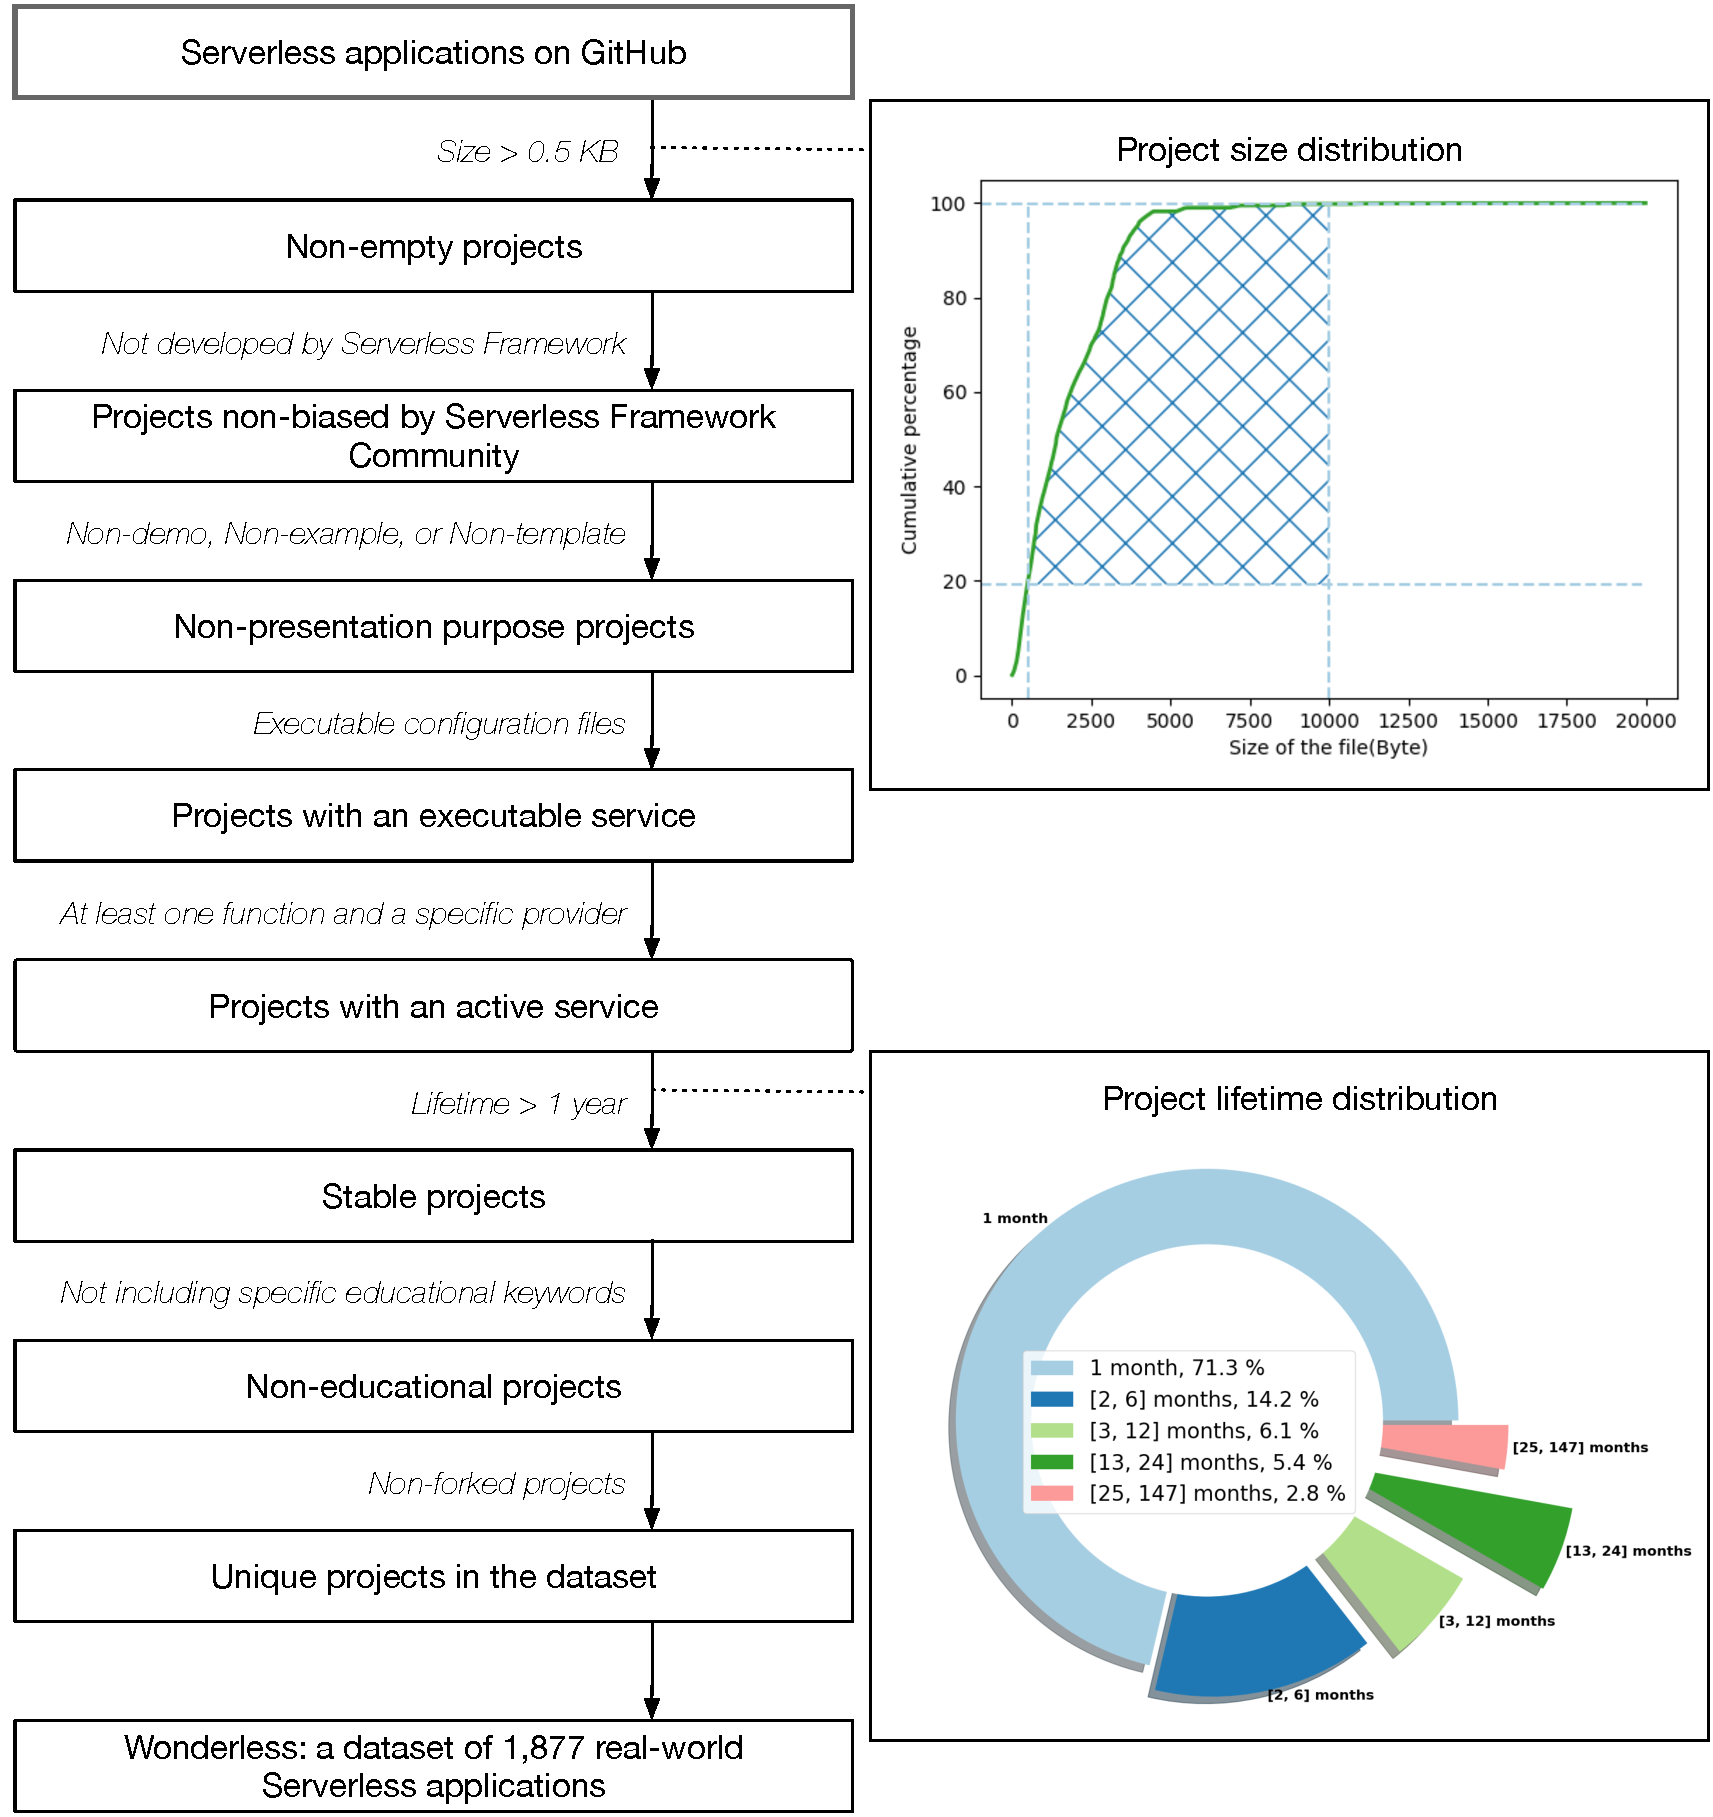
\includegraphics[scale=0.3]{figures/processOverviewFinalgraffle}
	\caption{Overview of creating Wonderless.}
	\label{fig:overview}
\end{figure}


Figure\,\ref{fig:overview} summarizes the  process of constructing Wonderless. 
The procedure consists of two main phases. 
We will thoroughly describe each of these phases in the following.

\subsection{Construction of the initial dataset} \label{phaseA}

To construct the initial dataset of Serverless applications, we chose GitHub projects 
devloped using the \emph{Serverless Framework}\,\footnote{\url{https://www.serverless.com}} 
-- we discuss this decision in section~\ref{discussion}.
This framework uses a default $serverless.yml$ configuration file, 
and it allows developers to deploy 
applications to cloud providers like AWS, Microsoft Azure, Google Cloud 
Platform, Apache OpenWhisk, Cloudflare Workers, or a Kubernetes-based 
solution like Kubeless.

Listing~\ref{lst:example} provides an example of a $serverless.yml$ file. 
Depending on the provider, this file can list different properties.
The example shows the configuration properties for a Telegram bot including 
name of the provider, runtime of the application, name of the function, 
and type of the event that triggers the function. 

We used the GitHub API to search for all the $serverless.yml$ files in GitHub. 
We broke down the query into subqueries based on the size of a file to 
overcome the limit of $1000$ results per query.
%Due to this, we searched for all the $serverless.yml$ files that are larger 
%than $0.5\,KB$ and smaller than $10\,KB$. The files with less than 
We discarded files smaller than $0.5\,KB$ which are mostly empty.
% and there are barely such files that are 
%larger than $10\,KB$. 
As the result of our search on July 29, 2020, 
we collected the URL of $41,862$ unique files, corresponded to 
$30,078$ repositories. Using the URLs, we cloned the main branch 
of repositories to create the initial version of the dataset resulting 
in $\sim400 \, GB$ of data.

\vspace{2mm}

\begin{lstlisting}[frame=single, caption=An example of a serverless.yml configuration file., label={lst:example}, captionpos=b]
service: azure-telegram-bot 

provider:  
		name: azure
		runtime: nodejs12.x  

plugins:  
		- serverless-azure-functions 

functions:
		hello:    
				handler: (*@handler.hello@*)
				events:   
						- http: true        
								x-azure-settings:          
										authLevel: anonymous
\end{lstlisting}

\subsection{Real-world Serverless applications} \label{phaseB}
The initial dataset includes a number of spurious data points 
such as inactive and toy projects. We then applied several rounds 
of filtering to the dataset.

As the first step to elude bias in the dataset, we checked the developers 
of the applications and removed a repository if it was developed 
by the \emph{Serverless Framework} community. Next, to remove the applications 
that served just as showcases, we removed a repository if the configuration file 
of the repository was placed in a directory that contained one of the 
\emph{example}, \emph{demo}, \emph{template}, or \emph{test} 
keywords in its label.

Then, 
%we used a python script to make an initial analysis of the 
%configuration files. We looked for the results of three metrics in this 
%analysis: 
we considered \rom{1}) if the configuration file is executable, \rom{2}) if 
the configuration file has the name of the provider property and 
\rom{3}) if the configuration file contains the information for any 
function. We removed a repository when the configuration file
does not meet any of these criteria. 
% if its configuration file was not 
% executable, had no particular provider, or had no specified function.
%
By the end of this step, the dataset had $371 \, GB$ of data consisting 
of $27,812$ unique repositories. 

To eliminate inactive projects, we removed a repositories with a lifetime 
(difference between the date of the last commit and the date of the first commit)
less than a year. 
% We used $git \; log$ to view the commit history of repositories. 
Figure~\ref{fig:overview} demonstrates the lifetime distribution of the 
projects in the dataset: more than $70\%$ of the projects 
were active for less than a month. Overall, more than $90\%$ 
of the project did not have a new commit a year after the initial one. 
This step dramatically reduced the size of the dataset to $2,364$ 
repositories.

To eliminate educational projects, 
we applied a keyword search to the labels, topics, and 
descriptions of repositories. We extracted the description 
and topics of each repository using the \emph{mercy-preview} media 
type of GitHub API previews. We removed a repository 
if the repository contained one of the following keywords: 
\emph{example, demo, tutorial, playground, learn, teach, exercise, 
	course, practice, template, sample, workshop, lecture, study}.

Finally, to avoid duplications, we removed a repository if it was forked 
or copied from other repositories in the dataset. To do this, we 
searched for the projects with the same name and different developers. 
Then we manually checked if those repositories were actually the same or 
they accidentally had the same name. If two repositories were the same, 
we removed the one with fewer commits or fewer contributors.





